%!TEX root = ../thesis.tex
%*******************************************************************************
%****************************** Second Chapter *********************************
%*******************************************************************************

\chapter{Simple 1-Dimentional Problem}

\ifpdf
    \graphicspath{{Chapter2/Figs/Raster/}{Chapter2/Figs/PDF/}{Chapter2/Figs/}}
\else
    \graphicspath{{Chapter2/Figs/Vector/}{Chapter2/Figs/}}
\fi


\section{Outlining of Basic Principles}

% Uncomment this line, when you have siunitx package loaded.
By constraining $\bm{x}$ to one dimention allows for the problem to be simplified. Suppose ${f(x)=\sin(x)+0.05x^2}$ with ${x\in [-10, 10]}$ as shown in Figure~\ref{fig:firstFunction}. In this range, there are multiple minima with only one global minima. The task here is to successfully locate the minima situated at -1.428 (found through ananlytical differentiation and solving ${10\cos(x)+x=0}$). This will be compared against two benchmarks: linear spacing and the fminbound method available in the scipy package given the same number of function calls. $\epsilon$ will be chosen to be independent of $x$ and $y$ and fit a normal distribution such that ${\epsilon\sim N(0, 0.2)}$.

\begin{figure}[htbp!] 
\centering    
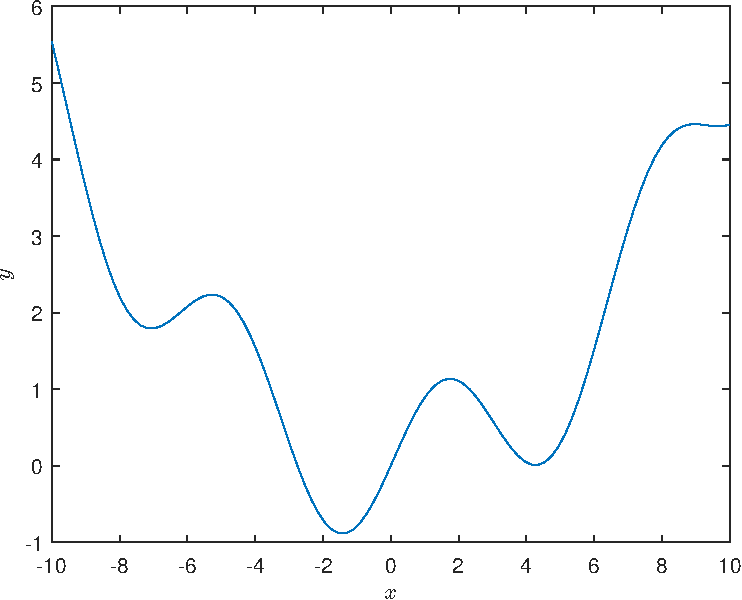
\includegraphics[width=1.0\textwidth]{firstFunction.pdf}
\caption[First Function]{$y = \sin(x) + 0.005x^2$ with $x\in [-10, 10]$}
\label{fig:firstFunction}
\end{figure}


\subsection{Algorithms}
\subsubsection{Linear Selection}
The least inteligent method while not being deliberately obtuse is linearly spacing sampled values and choosing $x$ equal to the lowest sampled value. This does have the advantage that all experimentations may be construed asynchronously. Thus, where material and labour cost is low, this may be beneficial.
\subsubsection{Active Learning}
This methodolgy has two underlying core principles: sparse areas reveal the most information and minimal areas reveal information to the location of the minima. Combining these allows for better decision making with regards to the next sample to choose.

There are several methods that may be used to enhance this strategy. Firstly, a smoothing spline between points allows for a non-parametric fit of the data to be used. Alternatively, a local regression fit may be used allowing for changes in sample density. Advanced methods using Baysian Statistics and advanced information theory may be used, although have been ommitted due to time restraints.

In this paper, three functions are found: $e(x)$, $p(x)$ and $h(x)$, denoting a guessed fit, the sparcity, and the height respectively. $p(x)$ is defined between adjacent samples, $s_i$.

\begin{equation}
  {h(x)=-e(x)+\max[e(x)]}
\end{equation}
\begin{equation}
  p(s_i \le x \le s_{i+1})=\min[x-s_i, s_{i+1}-x]
\end{equation}

The next sample is then taken as $\text{argmax}[h(x)p(x)]$.

\subsubsection{fminbound}
fminbound is a function included in the scipy optimisation library. It uses Brent's method allowing it to be quick in situations where labeling is quick and error is low.
\subsection[Comparison One]{Comparison on $\sin(x)+0.005x^2$}

Each method discussed in [] was executed 50 times for each sample size between 2 and 15. 

\begin{figure}[htbp!] 
  \centering    
  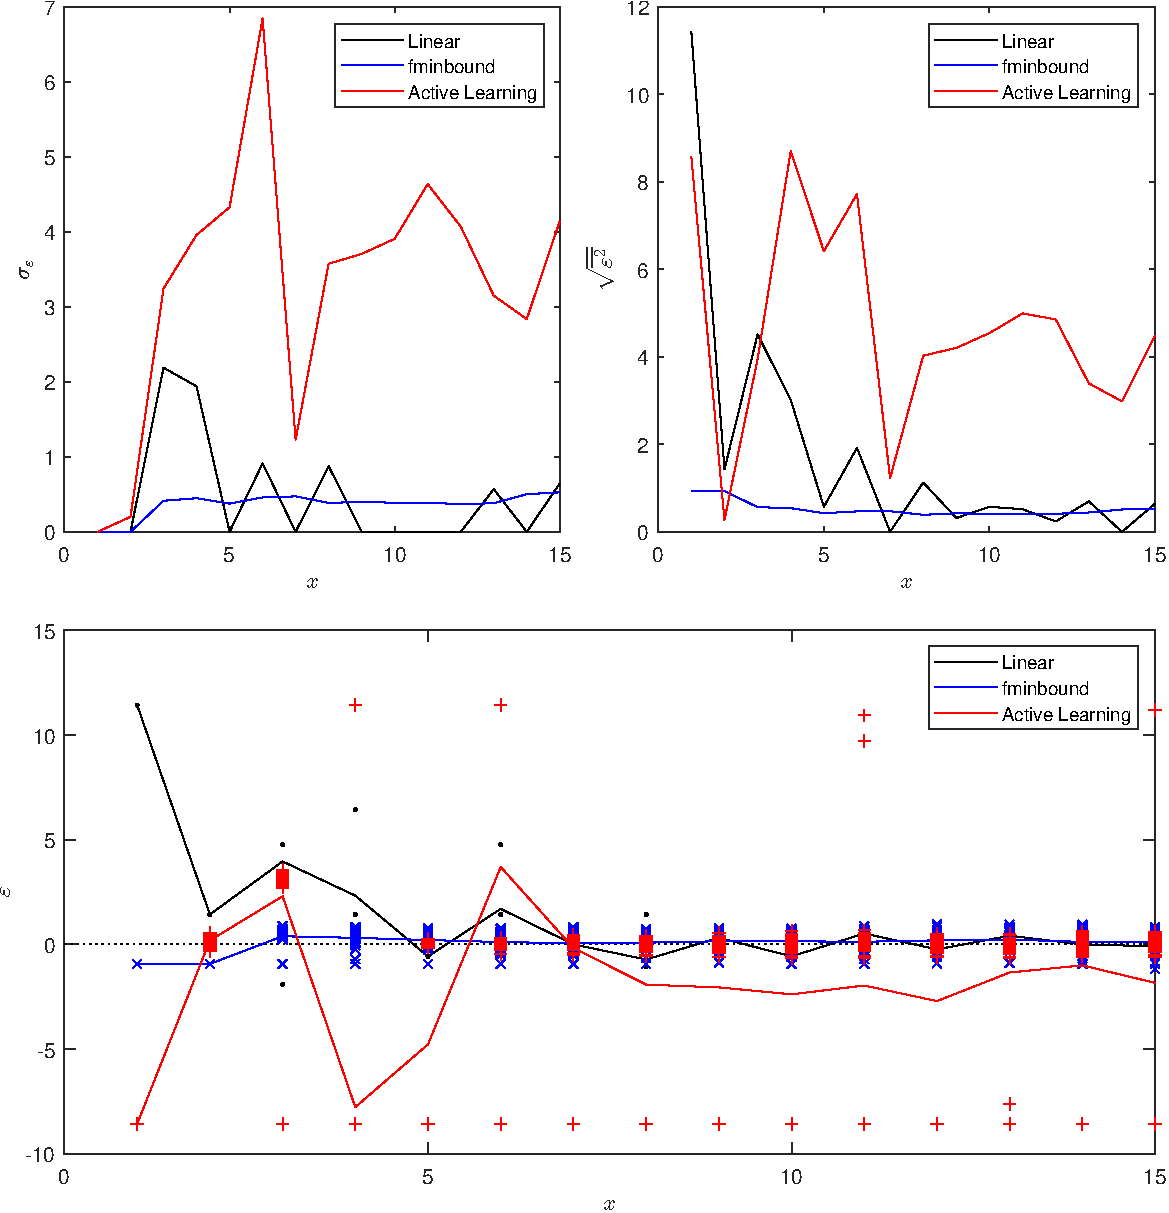
\includegraphics[width=1.0\textwidth]{comparison1.pdf}
  \caption[First Comparison]{Comparison of the three methods discussed. The top left shows the standard deviation of each method, the top right shows the square of the residues, and the bottom shows the result of each sample with an average of the residue drawn on to guide the eye.}
  \label{fig:firstComparison}
\end{figure}


\section*{Itemize}
\begin{itemize}
\item The first topic is dull
\item The second topic is duller
\begin{itemize}
\item The first subtopic is silly
\item The second subtopic is stupid
\end{itemize}
\item The third topic is the dullest
\end{itemize}

\section*{Description}
\begin{description}
\item[The first topic] is dull
\item[The second topic] is duller
\begin{description}
\item[The first subtopic] is silly
\item[The second subtopic] is stupid
\end{description}
\item[The third topic] is the dullest
\end{description}


\clearpage

\tochide\section{Hidden section}



\begin{landscape}

\section*{Subplots}
I can cite Wall-E (see Fig.~\ref{fig:WallE}) and Minions in despicable me (Fig.~\ref{fig:Minnion}) or I can cite the whole figure as Fig.~\ref{fig:animations}


\begin{figure}
  \centering
  \begin{subfigure}[b]{0.3\textwidth}
    
\includegraphics[width=\textwidth]{TomandJerry}
    \caption{Tom and Jerry}
    \label{fig:TomJerry}   
  \end{subfigure}             
  \begin{subfigure}[b]{0.3\textwidth}
    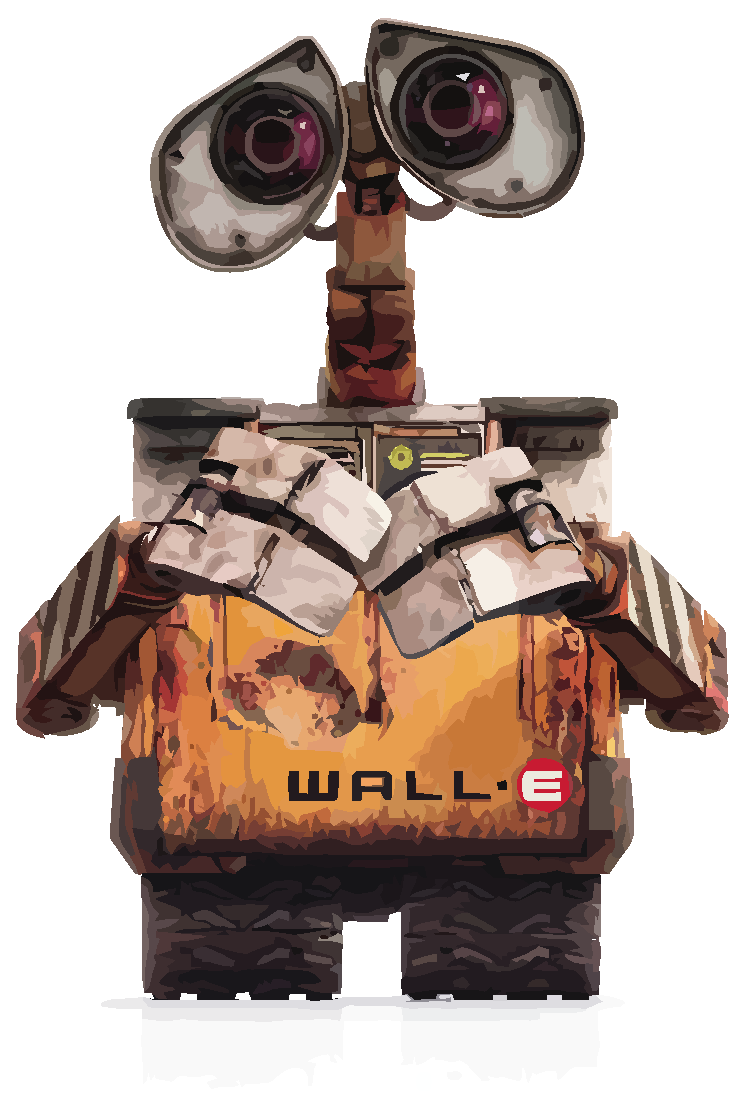
\includegraphics[width=\textwidth]{WallE}
    \caption{Wall-E}
    \label{fig:WallE}
  \end{subfigure}             
  \begin{subfigure}[b]{0.3\textwidth}
    
\includegraphics[width=\textwidth]{minion}
    \caption{Minions}
    \label{fig:Minnion}
  \end{subfigure}
  \caption{Best Animations}
  \label{fig:animations}
\end{figure}


\end{landscape}
